\documentclass{article}

\usepackage{graphicx}
\usepackage{tikz}
\usepackage{tikzsymbols}
\usetikzlibrary{calc,patterns,shapes.geometric}
\pagestyle{empty}
\usepackage[margin=0pt]{geometry}
\geometry{papersize={14in,12in}}

\def\centerarc[#1](#2)(#3:#4:#5){\draw[#1] ($(#2)+({#5*cos(#3)},{#5*sin(#3)})$) arc (#3:#4:#5);}

\begin{document}
	\begin{figure}
		\centering
		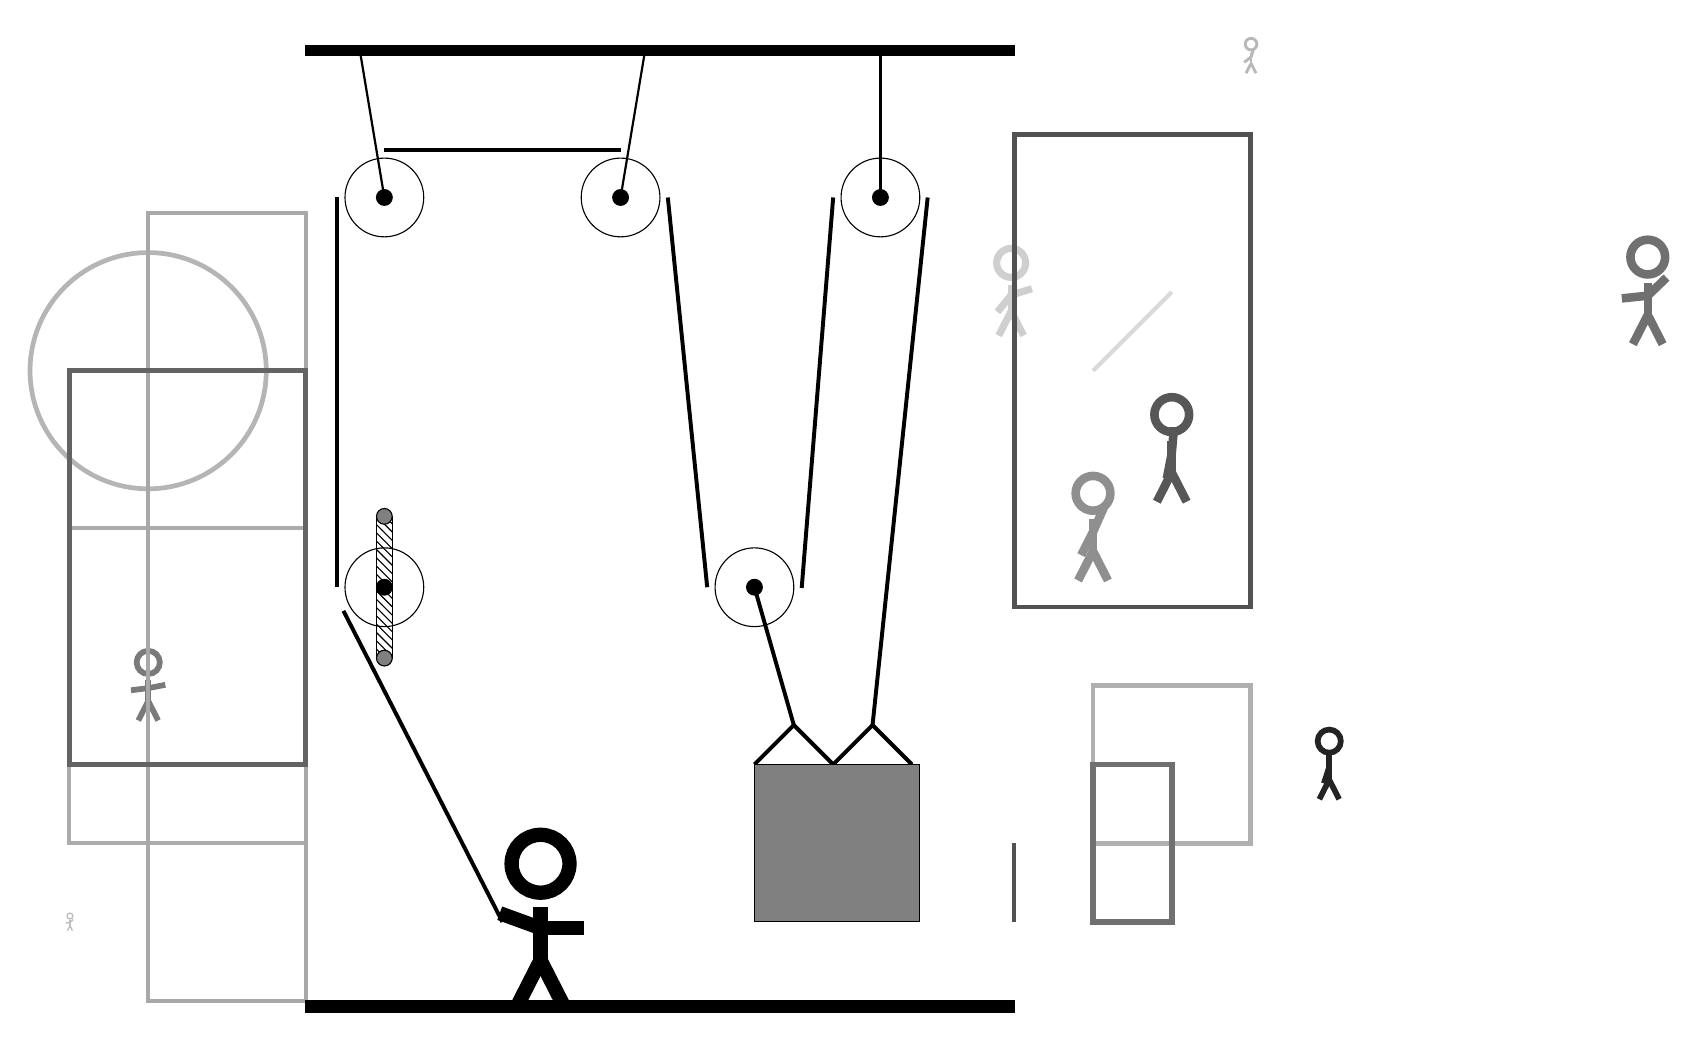
\begin{tikzpicture}
			%%%%% START %%%%%
			
			\draw[fill=black] (-3, 9) rectangle (6, 9.125);
			
			\draw (1, 7.2) circle (0.5);
			\draw[fill=black] (1, 7.2) circle (0.1);
			\draw[thick] (1, 7.2) -- (1.3, 9);
			
			\draw (4.3, 7.2) circle (0.5);
			\draw[fill=black] (4.3, 7.2) circle (0.1);
			\draw[thick] (4.3, 7.2) -- (4.3, 9);
			
			\draw[line width=0.6mm, color=black!31] (7, 1) rectangle (9, -1);
			
			\node[line width=0.5mm, color=black!52] at (-5, 1) {\Strichmaxerl[4][7][11]};
			\node[line width=0.6mm, color=black!19] at (6, 6) {\Strichmaxerl[5][51][17]};
			\draw[line width=0.5mm, color=black!33] (-3, 3) rectangle (-6, -1);
			\node[line width=0.7mm, color=black!56] at (14, 6) {\Strichmaxerl[6][6][44]};
			\draw[line width=0.5mm, color=black!15](7, 5) -- (8, 6);
			
			\draw [line width=0.6mm, color=black!29](-5, 5) circle (1.5);
			
			\node[line width=0.2mm, color=black!25] at (-6, -2) {\Strichmaxerl[1][6][43]};
			\node[line width=0.4mm, color=black!44] at (7, 3) {\Strichmaxerl[6][63][66]};
			\node[line width=0.3mm, color=black!86] at (10, 0) {\Strichmaxerl[4][72][90]};
			\draw[line width=0.7mm, color=black!56] (8, -2) rectangle (7, 0);
			\draw[line width=0.6mm, color=black!68] (6, 2) rectangle (9, 8);
			\draw[line width=0.5mm, color=black!34] (-5, -3) rectangle (-3, 7);
			
			\draw[line width=0.7mm, color=black!61] (-3, 5) rectangle (-6, 0);
			\draw[line width=0.5mm, color=black!68](6, -2) -- (6, -1);
			\node[line width=0.6mm, color=black!66] at (8, 4) {\Strichmaxerl[6][79][85]};
			\node[line width=0.6mm, color=black!28] at (9, 9) {\Strichmaxerl[2][38][72]};
			
			\draw (2.7, 2.25) circle (0.5);
			\draw[fill=black] (2.7, 2.25) circle (0.1);
			
			\draw[line width=0.5mm]  (2.7, 0) -- (3.2, 0.5) -- (3.7, 0) -- (4.2, 0.5) -- (4.7, 0);
			\draw[fill=black!50] (2.7, 0) rectangle (4.8, -2);
			
			\draw (-2, 7.2) circle (0.5);
			\draw[fill=black] (-2, 7.2) circle (0.1);
			\draw[thick] (-2, 7.2) -- (-2.3, 9);
			
			\draw (-2, 2.25) circle (0.5);
			\draw[fill=black] (-2, 2.25) circle (0.1);
			\draw[pattern=north west lines, pattern color=black] (-2.1, 3.15) rectangle (-1.9, 1.35);
			\draw[fill=black!50] (-2, 3.15) circle (0.1);
			\draw[fill=black!50] (-2, 1.35) circle (0.1);
			
			\draw[line width=0.5mm](-0.5, -2) -- (-2.5196, 1.95);
			\centerarc[line width=0.5mm](-2, 2.25)(180:210:0.6);
			\draw[line width=0.5mm](-2.6, 2.25) -- (-2.6, 7.2);
			\centerarc[line width=0.5mm](-2, 7.2)(90:180:0.6);
			
			\draw[line width=0.5mm](-2, 7.8) -- (1, 7.8);
			\centerarc[line width=0.5mm](1, 7.2)(0:90:0.6);
			\draw[line width=0.5mm](1.6, 7.2) -- (2.1, 2.25);
			\centerarc[line width=0.5mm](2.7, 2.25)(180:370:0.6);
			\draw[line width=0.5mm] (3.3, 2.24) -- (3.7, 7.2);
			\centerarc[line width=0.5mm](4.3, 7.2)(0:180:0.6);
			\draw[line width=0.5mm](4.2, 0.5) -- (4.9, 7.2);
			\draw[line width=0.5mm] (3.2, 0.5) -- (2.7, 2.25);
			
			\node at (0, -2) {\Strichmaxerl[10][-20][0]};
			
			\draw[fill=black] (-3, -3) rectangle (6, -3.15);
			
			%%%%% END %%%%%
		\end{tikzpicture}
	\end{figure}	
\end{document}